\chapter{Analysis challenges concerning \abbr{trna} expression data}
\label{sec:trna-analysis}

\section{Quantifying expression of \mrna genes}

In order to investigate protein-coding gene expression, we quantified the \mrna
abundance from \rrna-depleted \rnaseq data (strand-specific \SI{75}{bp}
paired-end reads from \name{Illumina} \name{HiSeq~2000}). Reads were mapped to
the \mmu reference genome (\abbr{ncbim37}) using \name{iRAP}
\citep{Fonseca:2014} and \name{TopHat2} \citep{Kim:2013}. Read counts were
quantified using \name{HTSeq} \citep{Anders:2014}, and assigned to
protein-coding genes from the \name{Ensembl} release \num{67}
\citep{Flicek:2014}.
\todo{add \chipseq and \rnaseq pipeline flowcharts}

We excluded mitochondrial chromosomes from the analysis, because mitochondrial
genes use a slightly distinct genetic code\todo{ref}. Furthermore, we excluded
sex chromosomes.

\section{Quantifying expression of \trna genes}

We quantified \trna gene expression via \pol3 \chipseq. The reason for using
this, on the first glance indirect, measure is caused by the fact that \trna
genes are unfortunately not identifiable by their sequence alone: performing a
multiple sequence alignment of \trna genes in \mmu reveals that several \trna
genes share the exact same sequence.

\todo{Fix alignment of table}
\textfloat{trna-alignment}{spill}
    {\footnotesize\begingroup
\let\m\mismatch
\begin{tabular}{@{}ll@{}}
    \toprule
    chr5.trna1044 &  \seq{GTCTCTGTGGCGCAATCGGTtAGCGCGTTCGGCTGTTAACCGAAAG...........GtTGGTGGTTCGAGCCCACCCAGGGACG}\\
    chr3.trna750 &   \seq{GTCTCTGTGGCGCAATCGGTtAGCGCGTTCGGCTGTTAACCGAAAG...........GtTGGTGGTTCGAGCCCACCCAGGGACG}\\
    chr3.trna298 &   \seq{GTCTCTGTGGCGCAATCGGTtAGCGCGTTCGGCTGTTAACCGAAAG...........GtTGGTGGTTCGAGCCCACCCAGGGACG}\\
    chr3.trna294 &   \seq{GTCTCTGTGGCGCAATCGGTtAGCGCGTTCGGCTGTTAACCGAAAG...........GtTGGTGGTTCGAGCCCACCCAGGGACG}\\
    chr3.trna289 &   \seq{GTCTCTGTGGCGCAATCGGTtAGCGCGTTCGGCTGTTAACCGAAAG...........GtTGGTGGTTCGAGCCCACCCAGGGACG}\\
    chr2.trna1947 &  \seq{GTCTCTGTGGCGCAATCGGTtAGCGCGTTCGGCTGTTAACCGAAAG...........GtTGGTGGTTCGAGCCCACCCAGGGACG}\\
    chr1.trna1014 &  \seq{GTCTCTGTGGCGCAATCGGTtAGCGCGTTCGGCTGTTAACCGAAAG...........GtTGGTGGTTCGAGCCCACCCAGGGACG}\\
    chr11.trna1446 & \seq{GTCTCTGTGGCGCAATCGGTtAGCGCGTTCGGCTGTTAACCGAAAG...........GtTGGTGGTTCGAGCCCACCCAGGGACG}\\
    chr10.trna390 &  \seq{GTCTCTGTGGCGCAATCGGTtAGCGCGTTCGGCTGTTAACCGAAAG...........GtTGGTGGTTCGAGCCCACCCAGGGACG}\\
    chr3.trna757 &   \seq{GTCTC\m CGTGGCGCAAT\m CGGT\m cAGCGCGTTCGGCTGTTAACCGAAAG...........GtTGGTGGTTCGAGCCCACCC\m GGGGACG}\\
    chr3.trna283 &   \seq{GTCTCTGTGGCGCAATTGGTtAGCGCGTTCGGCTGTTAACCGAAAG...........GtTGGTGGTTC\m AAGCCCACCCAGGGACG}\\
    \bottomrule
\end{tabular}
\endgroup
}
    {Alignment of Asn \trna genes.}
    {Parts of a multiple sequence alignment of \trna genes in \mmu generated
    with COVE\@. Shown are the \trna genes coding for Asn. Bases which differ
    from the consensus sequence are highlighted in red.}

In order to identify individual \trna genes and quantify their expression, we
therefore cannot resort to conventional \rnaseq: the \rna reads covering only
the transcribed gene region are indistinguishable.

With the \pol3 \chipseq data, we do not have this problem: reads cover both the
transcribed sequence and the flanking regions of each gene
(\cref{fig:trna-pol3-binding-profile}).

\textfig{trna-pol3-binding-profile}{spill}{\textwidth}
    {\trna \pol3 \chip binding profile.}
    {The shaded, bell-shaped area shows an idealised binding profile of \chipseq
    data spanning the \trna gene with the A and B box highlighted, as well as
    its flanking regions upstream and downstream of the gene body. This overlap
    plays a role in identifying the individual gene.}

When mapping the reads, we therefore do not discard all non-uniquely mapping
reads.\footnote{We still discard reads which are likely \pcr duplicates, i.e.\
map to many locations; we more or less arbitrarily used the threshold of
\num{20} non-unique mapping locations} We thus end up with reads which have not
been assigned to a given \trna gene (\cref{fig:trna-pol3-map-ambiguous-reads}).
In order to assign these reads to \trna genes, we \emph{reallocated} reads after
mapping, using the number of uniquely mapping reads in \trna genes’ flanking
regions to determine the most likely origin
(\cref{fig:trna-pol3-map-ambiguous-reads}) \citep{Kutter:2011}.

Formally, let \(i\) be the \(i\)th \trna gene locus, and \(c_i\) be the count of
uniquely mapped reads in its flanking region (we used \SI{\pm100}{bp}). A
multi-mapping read \(r\), which maps to a set \(T\) of candidate \trna[s], can
be allocated to a target \trna gene \(i\) randomly with probability

\begin{equation}
    p_i = \begin{cases}
        c_i\left(\sum_{x \in T}c_x\right)^{-1} &
            \text{if \(\sum_{x \in T}c_x \neq 0\),} \\
        \vert T \rvert^{-1} & \text{otherwise.}
    \end{cases}
\end{equation}

\textfloat{trna-pol3-map-ambiguous-reads}{spill}{%
    \centering
    \begingroup
        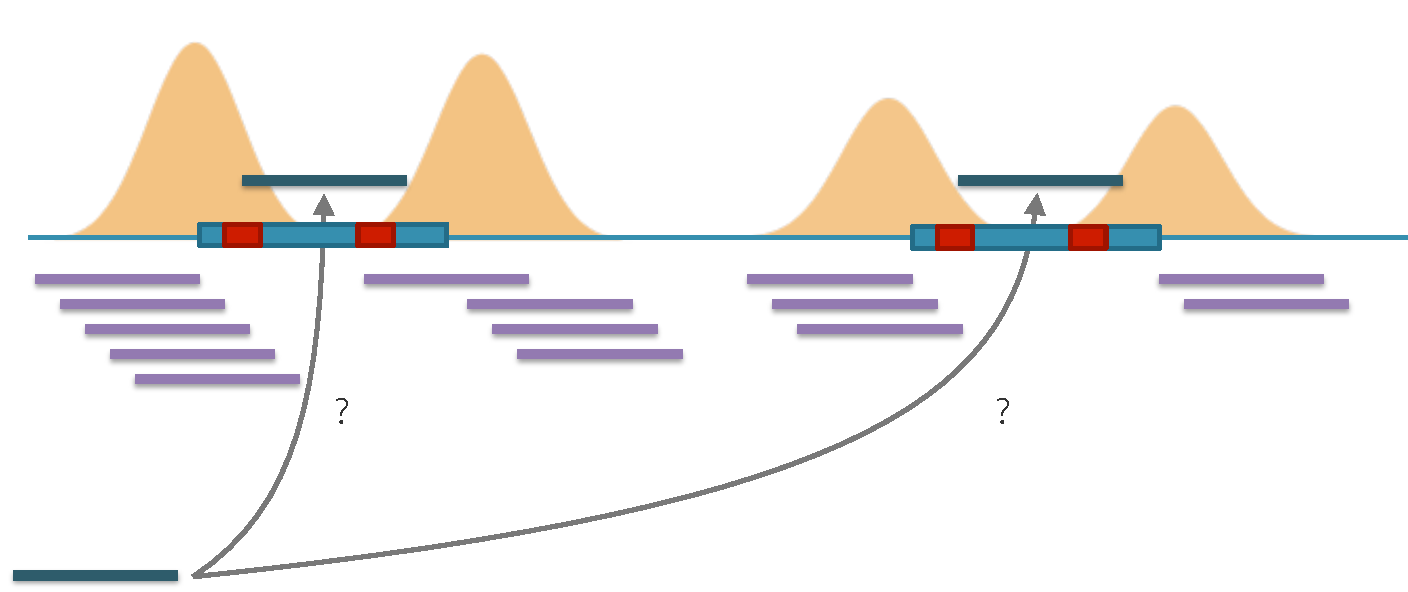
\includegraphics[width=\textwidth]{trna-pol3-map-ambiguous-reads-1}
        \subcaption{Two potential match candidate \trna genes for a read.}
    \endgroup
    \begingroup
        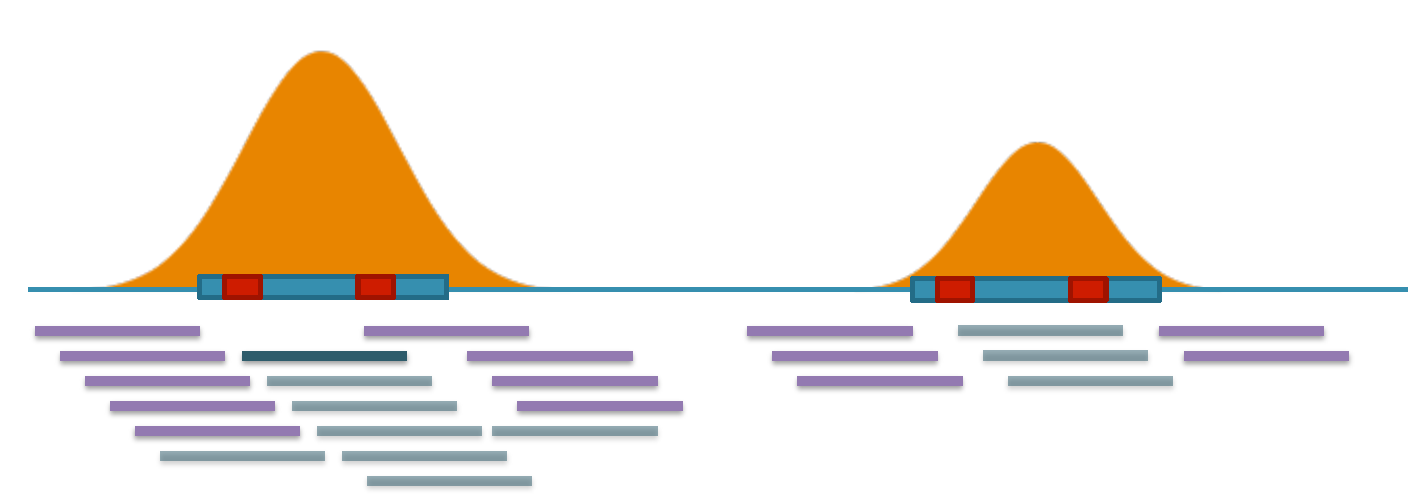
\includegraphics[width=\textwidth]{trna-pol3-map-ambiguous-reads-2}
        \subcaption{Using the count data from the flanking regions to
            extrapolate most likely mapping positions for ambiguous reads.}
    \endgroup}
    {Mapping ambiguous \chip reads.}
    {\chip reads originating from \trna genes can often not be mapped
    unambiguously to any given \trna. Instead, information form the gene’s
    flanking regions is used to determine the more likely provenance.}

Quantification of \trna genes was performed by first mapping the \pol3 \chipseq
data (non-strand-specific \SI{36}{bp} single-end reads sequenced by
\name{Illumina} \name{Genome Analyzer~IIx} or \name{HiSeq~2000}) using
\name{BWA} version 0.5.9-r16 \citep{Li:2009a} using default parameters. Next,
non-uniquely mapping reads were reallocated probabilistically according to the
description given above, using the \trna gene annotation from the \name{Genomic
\trna Database}, described in \citet{Chan:2009}. For each \trna gene (excluding
mitochondrial \trna genes), reads were summed on each \trna gene locus and in
the \SI{\pm100}{bp} flanking regions.

\trna genes that were unexpressed in all our experimental conditions were
excluded from the analysis, in order to reduce the effect of multiple testing,
and to exclude potential pseudogenes in the annotation. To be called expressed,
a \trna gene had to be present in all replicates of at least one condition with
a count of at least \num{10}, after size-factor normalisation. The threshold
\num{10} was chosen so that small variations in either direction would have a
minimal impact on the thresholding.

%\section{Normalisation of \trna gene expression}
%
%Raw \trna gene expression counts show strong differences between sequencing
%libraries. For \mrna count data, it is customary to use \name{DESeq}’s
%\dfn{library size normalisation} \citep{Anders:2010}. However, as shown in
%\cref{fig:trna-libraries-example}, library size normalised data still follows
%distinct distributions, which we deem biologically implausible, and probably due
%to technical bias.
%
%As a consequence, we opted to \dfn{quantile normalise} the count data\todo{find
%reference for quantile normalisation}.
%
%\textfloat{trna-libraries-example}{body}
%    {\centering\Huge Placeholder}{Placeholder}{Placeholder}

\section{Differential expression analysis}

\name{DESeq2} \citep{Love:2014} was used to call differentially expressed genes
for both \mrna and \trna genes between stages and tissues. In our analysis, we
called genes differentially expressed when their Benjamini–Hochberg
\fdr-corrected \(p\)-value was below \num{0.001}.

\section{PCA}

\todo{Write something about PCAs}

\section{Codon usage and correlation with anticodon abundance}

\subsection{Codon usage and anticodon abundance}

First, for every gene, the number of occurrences of each codon in the longest
annotated transcript (the “canonical” transcript) was determined and this value
was multiplied by the gene’s expression (normalised for transcript length).
Next, the overall usage of each codon was obtained by summing these values
across all genes. Relative codon and usage (excluding selenocysteine) were
calculated using

\begin{equation}
    x_{ij}^* = x_{ij}\left(\sum_{k=1}^n x_{kj}\right)^{-1},
\end{equation}

where \(x_ij\) is the triplet codon usage for triplet codon \(i\) in stage
\(j\), and \(x_{ij}^*\) is the relative usage.

Anticodon abundance was calculated by taking the mean of the expression values
for all \trna genes in a given anticodon isoacceptor family.

\subsection{Sampling background transcriptomes}

We used our library-size normalised \rnaseq and \pol3 \chipseq data to simulate
background distributions in liver and brain for each specific developmental
stage. We randomly rearranged the expression values across genes for the
expressed (\(e\)) and all genomically annotated (\(a\)) protein-coding genes and
\trna genes. For each developmental stage, we created \num{100} such random
background distributions. We then calculated triplet codon usage, as well as
isoacceptor abundance, for the rearranged protein-coding \rna and \trna
expression distributions.

\subsection{Correlating codon demand with anticodon supply}

In order to compare how well the anticodon supply of a given transcriptome was
adapted to its codon demand, we initially calculated the Spearman rank
correlation between the codon usage and the anticodon isoacceptor abundance.
Since not all codons have a corresponding anticodon-carrying \trna, unmatched
“orphan” triplet codons were discarded from the calculation.

The correlation coefficient thus calculated thus ignores the possibility of
wobble base pairing. In order to account for it, one could use an alternative
metric for how well adapted the \trna pool is to the codon pool
\citep{Gingold:2011}. In particular, \citet{Dos_Reis:2004} describe the \tai,
which takes into account all possible wobble base pairings when calculating the
fit between codon usage and anticodon abundance.\todo{Expand on tAI}

Rather than accounting for all possible base pairings, we opted for a simplified
version, in which non-orphan codons are matched with their directly
corresponding anticodons. Orphan codons were matched to the weighted sum of all
possible \trna anticodon isoacceptor matches by wobble base pairing. For this,
each anticodon isoacceptor abundance was weighted by estimating its probability
to pair with each possible codon.

To calculate correlations for the simulated transcriptomes, we first determined
the means for each of the \num{100} shuffled triplet codon distributions and
calculated their Spearman rank correlation with each of the \num{100} shuffled
isoacceptor distributions.

\section{Motif analysis}

The sequences of the \SI{500}{bp} upstream regions of differentially expressed
\trna genes between all pairwise stages in each tissue from the forward and
reverse strand were cleaned of low-complexity regions using the \name{dust}
application. A first-order Markov model built from the upstream regions of
all nondifferentially expressed \trna[s] in the appropriate stage–stage contrast
was used as background. Motif enrichment analysis in the sequences was conducted
with \name{MEME} \citep{Bailey:2009}, configured to search for zero or one
occurrences of one motif per sequence, up to a maximum of three distinct motifs,
with a minimum motif size of \SI{6}{bp}. Subsequently, \name{TOMTOM}
\citep{Gupta:2007} was used to interrogate the \name{MEME} output using the
input databases \identifier{JASPAR\_CORE\_2009\_vertebrates} and
\identifier{uniprobe\_mouse}. A minimum overlap of \SI{5}{bp} with an
\(E\)-value threshold of \num{10} was required.

\section{Colocalisation}

A test for colocalisation of the largest set of differentially expressed \trna
genes and differentially expressed \mrna genes was performed between
developmental stages (E15.5–P22 in liver and P4–P29 in brain). For each
up-regulated \trna gene \(i\), we counted the number of up-regulated
protein-coding genes, \(n_i\), and the total number of protein-codin genes,
\(b_i\), in the same genomic region of varying window sizes
(\SIlist{10;50;100}{kb}), which allowed us to compute the ratio \(r_i =
{n_i}/{b_i}\). We repeated this analysis for each non-differentially
expressed \trna gene \(j\) to obtain the ratio \(r_j^*\). A Kolmogorov–Smirnov
test was performed to assess whether the distribution \(r\) of ratios of
up-regulated protein-coding genes was significantly different in the vicinity of
up-regulated \trna genes from the distribution \(r^*\) in the vicinity of
nondifferentially expressed \trna genes with varying significance thresholds
(\numlist{0.1;0.05;0.01}).

\section{Chromatin association}

Publicly available \chipseq data of histone marks (\geo accession
\identifier{GSE29184}) associated with genomic regions at promoters and
enhancers (H3K4me3, H3K4me1, H3K27ac), \pol2, and an insulator (\ctcf)
\citep{Shen:2012} were used to assess whether any of these marks were associated
(Fisher’s exact test) with

\begin{enumerate}
    \item active versus inactive \trna genes in embryonic (E15.5) and adult
        (P29) tissues; and
    \item differentially expressed \trna genes between E15.5 and P29
\end{enumerate}

in mouse liver and brain tissues. Occurrence of these chromatin marks was
measured \SIlist{0.1;0.5;1}{kb} upstream of and downstream from \trna genes. Our
embryonic (E15.5) and adult (P29) \pol3 data was complemented with embryonic
(E14.5) and adult (P56) \chipseq data, as different time points were selected in
our and in the \citet{Shen:2012} study. Likewise, our brain P29 data was
compared with P56 data by merging “cortex” and “cerebellum” \chipseq data from
\citet{Shen:2012}.

\section{Compensation}

For each isoacceptor that is encoded by more than two \trna genes, we calculated
Spearman’s rank correlation (across developmental stages) between the expression
values of each pair of its corresponding \trna genes, i.e.\ we calculate

\begin{equation}
    c_{ij} = \operatorname{Cor}(x_i, x_j) \text{ for \(i, j \in T, i < j\)},
\end{equation}

where \(T\) is the set of \trna genes in the isoacceptor family, and \(x_i\) is
the vector of expression values of the \(i\)th \trna gene across all stages of
development. For the same set of genes, we calculated a null set of correlations
as follows:

\begin{equation}
    b_{ijk} = \operatorname{Cor}(\operatorname{perm}_k(x_i), x_j)
        \text{ for \(i, j \in T, i < j; k \in 1\dots\lvert x_i\rvert!\)}.
\end{equation}

Here, \(\operatorname{perm}_k(x_i)\) is the \(k\)th permutation of the vector
\(x_i\).

Next, we used the \(\chi^2\)-test to investigate whether there was a significant
difference between the background \(b\) and the observed correlation
distributions \(c\). We reported the Bonferroni-corrected \(p\)-value for the
\num{27} isoacceptor families with six or more genes, since isoacceptor families
with less than six genes did not enough points for meaningful interpretation.

\section{Genomic clusters}

We defined \num{69} clusters of all genomically annotated \trna genes that lie
within \SI{7.5}{kb} of each other. We counted how many active \trna genes of an
isoacceptor family colocalised in a genomic cluster with \trna genes of the same
isoacceptor family. We calculated the fraction of \trna for each isoacceptor
family belonging to a genomic cluster. In order to test whether genes in
isoacceptor families tend to genomically colocalise more than expected by
chance, we randomly assigned \trna genes to isoacceptor families (preserving the
actual isoacceptor family gene numbers) \num{1000} times. We then tested whether
the mean percentage of clustering \trna genes per isoacceptor family differed
from the mean percentage expected by chance, by using a binomial test. Finally,
we tested whether there wa a difference in these percentages between isoacceptor
families that show evidence for compensation, and isoacceptor families that show
no such evidence by applying a \(\chi^2\)-test.

\section{An overview over failed analysis approaches}
